\documentclass[unicode,11pt,a4paper,oneside,numbers=endperiod,openany]{scrartcl}

\usepackage{ifthen}
\usepackage[utf8]{inputenc}
\usepackage{graphics}
\usepackage{graphicx}
\usepackage{hyperref}

\pagestyle{plain}
\voffset -5mm
\oddsidemargin  0mm
\evensidemargin -11mm
\marginparwidth 2cm
\marginparsep 0pt
\topmargin 0mm
\headheight 0pt
\headsep 0pt
\topskip 0pt        
\textheight 255mm
\textwidth 165mm

\newcommand{\duedate} {}
\newcommand{\setduedate}[1]{%
\renewcommand\duedate {Due date:~ #1}}
\newcommand\isassignment {false}
\newcommand{\setassignment}{\renewcommand\isassignment {true}}
\newcommand{\ifassignment}[1]{\ifthenelse{\boolean{\isassignment}}{#1}{}}
\newcommand{\ifnotassignment}[1]{\ifthenelse{\boolean{\isassignment}}{}{#1}}

\newcommand{\assignmentpolicy}{
\begin{table}[h]
\begin{center}
\scalebox{0.8} {%
\begin{tabular}{|p{0.02cm}p{16cm}|}
\hline
&\\
\multicolumn{2}{|c|}{\Large\textbf{HPC Lab 2020 ---  Submission Instructions}}\\
\multicolumn{2}{|c|}{\large\textbf{(Please, notice that following instructions are mandatory: }}\\
\multicolumn{2}{|c|}{\large\textbf{submissions that don't comply with, won't be considered)}}\\
&\\
\textbullet & Assignments must be submitted to \href{https://www.icorsi.ch/course/view.php?id=10049}{Icorsi} (i.e. in electronic format).\\
\textbullet & Provide both executable package and sources (e.g. C/C++ files, Matlab). 
If you are using libraries, please add them in the file. Sources must be organized in directories called:\\
\multicolumn{2}{|c|}{\textit{Project\_number\_lastname\_firstname}}\\
& and  the  file must be called:\\
\multicolumn{2}{|c|}{\textit{project\_number\_lastname\_firstname.zip}}\\
\multicolumn{2}{|c|}{\textit{project\_number\_lastname\_firstname.pdf}}\\
\textbullet &  The TAs will grade your project by reviewing your project write-up, and looking at the implementation 
                 you attempted, and benchmarking your code's performance.\\

\textbullet & You are allowed to discuss all questions with anyone you like; however: (i) your submission must list anyone you discussed problems with and (ii) you must write up your submission independently.\\
\hline
\end{tabular}
}
\end{center}
\end{table}
}
\newcommand{\punkte}[1]{\hspace{1ex}\emph{\mdseries\hfill(#1~\ifcase#1{Points}\or{Points}\else{Points}\fi)}}


\newcommand\serieheader[6]{
\thispagestyle{empty}%
\begin{flushleft}

\includegraphics[width=0.4\textwidth]{images/usi_inf.pdf}
\end{flushleft}
  \noindent%
  {\large\ignorespaces{\textbf{#1}}\hspace{\fill}\ignorespaces{ \textbf{#2}}}\\ \\%
  {\large\ignorespaces #3 \hspace{\fill}\ignorespaces #4}\\
  \noindent%
  \bigskip
  \hrule\par\bigskip\noindent%
  \bigskip {\ignorespaces {\Large{\textbf{#5}}}
  \hspace{\fill}\ignorespaces \large \ifthenelse{\boolean{\isassignment}}{\duedate}{#6}}
  \hrule\par\bigskip\noindent%  \linebreak
 }

\makeatletter
\def\enumerateMod{\ifnum \@enumdepth >3 \@toodeep\else
      \advance\@enumdepth \@ne
      \edef\@enumctr{enum\romannumeral\the\@enumdepth}\list
      {\csname label\@enumctr\endcsname}{\usecounter
        {\@enumctr}%%%? the following differs from "enumerate"
	\topsep0pt%
	\partopsep0pt%
	\itemsep0pt%
	\def\makelabel##1{\hss\llap{##1}}}\fi}
\let\endenumerateMod =\endlist
\makeatother




\usepackage{textcomp}





\begin{document}


\setassignment
\setduedate{27.11.2020 23:59 (midnight)}

\serieheader{High-Performance Computing Lab}{Fall 2020}{Student: Gabriele Berra}{Discussed with: -}{Solution for Project 6}{}
\newline

\assignmentpolicy

\section{Ring maximum using MPI [10 Points]}
In this first exercise I implemented the function \textit{max\_ring.c} parallelized with MPI. Similarly to what we did in class I firstly define the left and right neighbour and the value of the function  
\begin{equation}\label{eq:maxEx1}
	\text{max} = 3 * \text{process\_rank}_i \mod(2 * \text{communicator\_size}) 
\end{equation}
for each processor. Since we have to run the function with 4 processors we know that the global maximum of Eq. \ref{eq:maxEx1} is reached in the processor 2 with $\max = 6$. In the main body of the function, on one hand, each processor, with the MPI routine MPI\_Send, exchanges its own maximum with the next processor. On the other hand, with the MPI routine MPI\_Recv, the processor that receive the data check if its own maximum is bigger or lower than the maximum that it has received and keeps the bigger one. Repeating this routine in a circular manner 4 times gives the following results:

\begin{lstlisting}[language = bash, backgroundcolor=\color{gray!20}]
Process 0:		Max = 6
Process 2:		Max = 6
Process 3:		Max = 6
Process 1:		Max = 6
\end{lstlisting}
 Of course, every time we run the script the order of the processes will change. In what follows I reported the main body of the function \textit{max\_ring.c}.

\lstinputlisting[frame=single, breaklines=true, tabsize=3, showstringspaces=false, firstline=53 ,lastline=71, language=C]{code/max_ring.c}


\section{Ghost cells exchange between neighboring processes [20 Points]}
For this second exercise we have to parallelize wit MPI the exchange of "ghost cells" between adjacent processors in a defined grid. The input data on which we have to work is a $(6+2)\times(6+2)$ matrix associated with each processors in which each entries has value equal to the rank of the processor. 
The first step is to create a Cartesian communicator of dimension $4\times 4$ (which is a sort of matrix for the processors) with periodic boundaries, which means that the processor 0 - which is in position $(0,0)$ - can communicate with processor 3 and processor 12 on the left and top respectively. In order to find, for each processors, the top, bottom, left and right neighbour we have to use the MPI routine MPI\_Cart\_shift which, given a shift direction and the amount of "cells" to be shifted, returns the source and destination rank. In our case, to find the left and right neighbour we use:

\lstinputlisting[frame=single, breaklines=true, tabsize=3, showstringspaces=false, firstline=92 ,lastline=92, language=C]{code/ghost.c}
which shifts on the $x$ axis (second input) of 1 cell (third input). Similarly, to find the top and bottom neighbour we use:
\lstinputlisting[frame=single, breaklines=true, tabsize=3, showstringspaces=false, firstline=93 ,lastline=93, language=C]{code/ghost.c}
which, in this case, shifts on the $y$ axis - vertically - of 1 cell.\\ Now that we know the neighbourhood of each processor we have to exchange the correct data between them. We know that, since C stores data in row-major order, we have no problem in exchanging rows of a matrix because the data are contiguous in memory. The problem occurs when we want to exchange data that are not contiguous in memory. Fortunately MPI gives us the routine MPI\_Type\_vector which can create a vector-type object. In order to use it in the correct manner we first have to understand how it works. As input it accepts:

\begin{itemize}
	\item \textit{count}: number of blocks that we want to send;
	\item \textit{blocksize}: dimension of the block (in our case, since we want to sent only double, is equal to 1);
	\item \textit{stride}: distance in memory between elements that we want to send;
	\item \textit{type}: type of the item that we want to send.
\end{itemize}

The last element in MPI\_Type\_vector is the output. Now we have created only a structure without any data inside it. When we use it in MPI\_Send, what it does is to take \textit{count} elements with distance from each other equal to \textit{stride}.\\ The last step is the exchange of the correct data between neighbours. To do so I used the MPI routine MPI\_Send and MPI\_Recv in which, for each processor, I specify the correct position of the data that has to be sent and the position in which the receiver has to put the data received. As explained before, I used the vector-type object only to exchange data between left and right neighbours. The code I implemented is the following:\\
\lstinputlisting[frame=single, breaklines=true, tabsize=3, showstringspaces=false, firstline=101 ,lastline=121, language=C]{code/ghost.c}


\section{Parallelizing the Mandelbrot set using MPI [20 Points]}
With the aim of creating the mandelbrot set using MPI I firstly implemented the functions \textit{createPartition()}, \textit{updatePartition()} and \textit{createDomain()} in the file \textit{consts.h} as follows:
\lstinputlisting[frame=single, breaklines=true, tabsize=3, showstringspaces=false, firstline=43 ,lastline=135, language=C]{code/consts_mandel.h}

\begin{figure}[h!]
	\hspace{-1.5cm}\includegraphics[width=0.7\textwidth, angle=-90]{images/perf.ps}
	\vspace{1cm}
	\caption{Performance with different amount of processors}
	\label{fig:mandelPerf}
\end{figure}

As we can see in figure \ref{fig:mandelPerf} the time for the computation of the mandelbrot set using two processors is halved compared to the time using only one processors. In contrast, the differences between the time using 4 processors and the time using 8 processors is almost the same. We can notice that the computation time of, as example, the processor 5, in the run using 16 processes, is exactly equal to the computational time of processor 9. This comparison can be extended to all the processes. The reason for this behaviour lies in the symmetry, with respect to the x axis, of the mandlebrot set. Thus, in a $4 \times 4$ grid reported in the left side of Fig.\ref{fig:procMatrix} the pairs of processors with the same computational time are: (0 - 12), (1 - 13), (2 - 14), (3 - 15), (4 - 8),(5 - 9),(6 - 10) and, (7 - 11). We know that different areas of the mandelbrot set require different amount of time to compute. In my opinion, the most interesting aspect - which is also the explanation of why this method of partitioning is not the most efficient - is the difference in terms of computational time between different processes. One of the most efficient way to parallelize the mandelbrot set is to distribute the work among the processes in an equal way in terms of computational time.
\begin{figure}[h!]
	\centering
	\begin{subfigure}[b]{0.48\textwidth}
		\hspace{3cm}\begin{tikzpicture}
		\matrix[matrix of nodes,nodes={draw=gray, anchor=center, minimum size=1cm}, column sep=-\pgflinewidth, row sep=-\pgflinewidth] (A) {
		\Large{0} & \Large{1} & \Large{2} & \Large{3} \\
		\Large{4} & \Large{5} & \Large{6} & \Large{7} \\
		\Large{8} & \Large{9} & \Large{10} & \Large{11} \\
		\Large{12} & \Large{13} & \Large{14} & \Large{15}\\};
		\end{tikzpicture}
	\end{subfigure}
	\hfill
	\begin{subfigure}[b]{0.48\textwidth}
		
\includegraphics[width=0.53\textwidth]{images/mandel.png}
	\end{subfigure}
	\caption{Mandelbrot set}
	\label{fig:procMatrix}
\end{figure}


\section{Option A: Parallel matrix-vector multiplication and the power method [50 Points]}




\end{document}
